\documentclass[10pt,a4paper,twocolumn]{article}
\usepackage[utf8]{inputenc}
\usepackage[T1]{fontenc}
\usepackage[spanish,es-noquoting]{babel}
\usepackage{lmodern,microtype}
\usepackage{amsmath,amssymb,amsthm,bm}
\usepackage{graphicx,booktabs,tabularx,array,longtable,multicol}
\usepackage[dvipsnames]{xcolor}
\usepackage{tikz}
\usetikzlibrary{positioning,arrows.meta,shapes.geometric,fit,calc}
\usepackage{enumitem}
\usepackage[breaklinks=true,colorlinks=true,urlcolor=NavyBlue,citecolor=NavyBlue,linkcolor=NavyBlue]{hyperref}
\usepackage[margin=18mm,top=20mm,bottom=20mm,columnsep=7mm]{geometry}
\usepackage{fancyhdr}
\usepackage{tcolorbox}
\usepackage{float}
\usepackage{balance}
\definecolor{ink}{HTML}{19304B}
\definecolor{accent}{HTML}{137D91}
\definecolor{papergray}{HTML}{EFF4F7}
\definecolor{orange}{HTML}{B55B25}
\renewcommand{\baselinestretch}{1.0}
\setlength{\parindent}{0.85em}
\setlength{\parskip}{0pt}
\setlist[itemize]{leftmargin=*,itemsep=1pt,topsep=2pt}
\setlist[enumerate]{leftmargin=*,itemsep=2pt,topsep=2pt}
\pagestyle{fancy}
\fancyhf{}
\fancyhead[L]{\footnotesize\color{ink}PABe-CBF --- Evaluación en simulación}
\fancyhead[R]{\footnotesize\color{ink}Octubre de 2026}
\fancyfoot[C]{\footnotesize\thepage}
\renewcommand{\headrulewidth}{0.4pt}
\newtheorem{theorem}{Teorema}
\newtheorem{proposition}{Proposición}
\newtheorem{remark}{Observación}
\newcommand{\bvec}{\mathbf{b}}
\newcommand{\RR}{\mathbb{R}}
\newcommand{\calC}{\mathcal{C}}
\newcommand{\calU}{\mathcal{U}}
\newcommand{\calW}{\mathcal{W}}
\newcommand{\calV}{\mathcal{V}}
\newcommand{\subttl}[1]{\vspace{3pt}\noindent\textbf{\color{ink}#1.}~}
\newcommand{\arxiv}[1]{\href{https://arxiv.org/abs/#1}{arXiv:#1}}
\newcommand{\doi}[1]{\href{https://doi.org/#1}{DOI \textsf{[enlace]}}}
\newcommand{\notehead}[1]{\vspace{2pt}\noindent\textbf{\color{ink}#1}\enspace}
\title{\bfseries\color{ink}PABe-CBF: evaluación en simulación\\[-2pt]
\large\normalfont\color{accent}Sección de resultados (documento autónomo de revisión)}
\author{\small Generado con el paquete \texttt{pabe\_cbf}}
\date{\small Octubre de 2026}
% Etiquetas del manuscrito principal referidas desde esta sección
\makeatletter
\newcommand{\fakelabel}[2]{\protected@write\@auxout{}{\string\newlabel{#1}{{#2}{}{}{}{}}}}
\makeatother
\begin{document}
\fakelabel{eq:qp}{9}\fakelabel{eq:hmm}{2}\fakelabel{eq:zeroevents}{16}
\maketitle
% ============================================================================
% Sección de evaluación en simulación para el manuscrito PABe-CBF.
% Generada a partir de results/paper/exp.pkl (pabe_cbf.paper_exp / paper_figs).
% Requiere: graphicx, booktabs, amsmath. Figuras en figures/, tablas en tables/.
% ============================================================================
\section{Evaluación en simulación}
\label{sec:sim}

\subsection{Banco de pruebas}
\label{sec:sim:setup}
Para someter la propuesta a una primera prueba falsable se implementó un banco de
pruebas abierto y reproducible (paquete \texttt{pabe\_cbf}). Por razones de alcance es
una \emph{abstracción planar} del apretón de manos y \emph{no} un gemelo digital del
Unitree~G1. El brazo del robot es una cadena de 3~GDL con longitudes de 0{,}30/0{,}28/0{,}10\,m y control
de velocidad articular ($|u_i|\le 2{,}5$\,rad/s), que representa la salida del
controlador de cuerpo completo. La perturbación articular está acotada:
$|w_i|\le 0{,}03$\,rad/s, con $0{,}10$\,rad/s en la familia de perturbación, por encima de la cota de
diseño $0{,}05$\,rad/s. El brazo humano sigue un guion de lazo abierto
con perfiles de mínimo \emph{jerk}, idéntico para todos los métodos por semilla. El
contacto se modela como un resorte de agarre ($K=300$\,N/m). Los puntos controlados son
el codo, el antebrazo, la muñeca y la palma, con barreras de distancia por eslabón frente a la
mano, la muñeca, el codo y el torso humanos ($d^{\rm phys}=6$\,cm). Se usa $F_{\rm phys}=20$\,N y
$F_{\rm soc}=12$\,N. Las estimaciones tienen cotas de error demostrables:
$\epsilon_d=1{,}5$\,cm, $\epsilon_v=0{,}10$\,m/s y $\epsilon_F=0{,}6$\,N. Durante una oclusión,
la cota crece como el conjunto alcanzable con velocidad inicial conocida y
aceleración acotada (1{,}5\,m/s$^2$). El lazo CBF corre a 100\,Hz y el HMM a
33\,Hz. El QP~\eqref{eq:qp} se resuelve con \texttt{quadprog} (Goldfarb--Idnani).

Las observaciones son sintéticas: velocidad radial visual, una señal proxémica de
disposición y una señal táctil de agarre, esta última solo en contacto. Incluyen un transitorio
ambiguo al establecer el contacto. El HMM~\eqref{eq:hmm} se ajusta por máxima
verosimilitud supervisada, con matrices $A^{(m)}$ por grupo de modo y emisiones $t$ de
Student ($\nu=4$, posición mediana, escala MAD). $H_{\rm ref}(m,\tau)$ es el
cuantil~0{,}8 de la entropía en trazas nominales. La cota $p_W^+$ se obtiene por
regresión isotónica de $b_W$ con una cota superior de Clopper--Pearson por bloque. El
tamaño efectivo de cada bloque se cuenta como el número de \emph{episodios} distintos y no de
ticks, porque los ticks de un episodio están autocorrelacionados.

\subttl{Particiones y protocolo} Todos los conjuntos son disjuntos por participante
simulado:
\begin{itemize}
\item entrenamiento del HMM y de $H_{\rm ref}$: 12 participantes;
\item calibración de $p_W^+$, del cuantil conforme de B5 y del umbral de B8: 10 participantes;
\item validación, usada solo para elegir umbrales: 10 participantes;
\item test: 20 participantes $\times$ 6 familias $\times$ 5 semillas, es decir, 600 episodios por método.
\end{itemize}
El 25\,\% de los participantes de validación y de test presenta cambio de dominio, con señales
de disposición atenuadas y más ruidosas. B3, B5 y B9 se comparan \emph{a igual sensibilidad}. En validación se
barrió el umbral de liberación y se eligió, para cada método, el de menor cancelación falsa
que detecta al menos $s^\star=80$\,\% de las retiradas en $\le1$\,s. Las
variantes que comparten la regla de B9 (B6, A1--A7) usan el mismo umbral, y B2, B4, B7 y B8
conservan su regla nativa. En total se simularon 27\,000 episodios de test.

\subttl{Transparencia sobre el desarrollo} Durante el desarrollo se evaluó una versión
previa (v1) sobre otra partición de test. En ella se observaron dos defectos de
especificación que afectaban a todos los métodos con HMM:
(i) con emisiones gaussianas, el estado W, que mezcla ``retirándose'' y ``ya
retirado en reposo'', quedaba mal representado, y la creencia volvía a H con la mano quieta;
(ii) la cota $p_W^+$ por bins aplanaba el orden de las probabilidades.
Ambos se corrigieron antes de los resultados aquí reportados, que se obtuvieron sobre una partición de
test \emph{nueva} (participantes 4000+) que no intervino en ninguna decisión. La
variante v1 de la calibración se conserva como ablación A8.

\subttl{Análisis estadístico} Las tasas por episodio llevan IC~95\,\% de
Clopper--Pearson. Cuando no hay eventos se informa además la cota unilateral
de la Ec.~\eqref{eq:zeroevents}. Los contrastes pre-registrados (Tabla~\ref{tab:contrasts})
usan bootstrap pareado por episodio, remuestreando \emph{participantes} (4000 réplicas), y la
familia completa de nueve contrastes se corrige con Holm.

\subsection{Resultados globales}
\label{sec:sim:main}
La Tabla~\ref{tab:main} y la Fig.~\ref{fig:methods} resumen los diez comparadores.
\begin{itemize}
\item \textbf{Violaciones.} Sin filtro (B0), el 54{,}8\,\% de los episodios presenta al menos una violación
física, sobre todo contacto no autorizado de la palma (47{,}3\,\%). Con el CBF de umbrales
fijos (B1) la tasa baja al 4{,}3\,\%, toda por exceso de fuerza en retiradas
durante el contacto y bajo perturbaciones que exceden la cota de diseño (18\,\% en la
familia~vi; Tabla~\ref{tab:families}). B9 no registró violaciones en 600 episodios. Esto acota la tasa por
debajo de 0{,}5\,\% (unilateral 95\,\%) bajo el supuesto i.i.d., lo que \emph{no} equivale a riesgo nulo.
\item \textbf{Retirada.} Los métodos sin regla semántica de retirada (B1 y B7) fallan la
liberación en el 15{,}7\,\% y el 19{,}3\,\% de las retiradas con contacto. B9 no falla ninguna (IC
[0, 2{,}3]\,\%). Con todo, B2--B6 obtienen el mismo resultado.
\item \textbf{Tarea.} B9 completa el 93{,}7\,\% de los apretones autorizados, con un 6{,}3\,\% de cancelaciones
falsas [3{,}9, 9{,}7]. Las cancelaciones falsas se concentran en las familias de duda inocua y de
oclusión. En oclusión la causa es la expansión del conjunto alcanzable, común a todos
los métodos filtrados.
\end{itemize}

\begin{figure*}[!t]
\centering
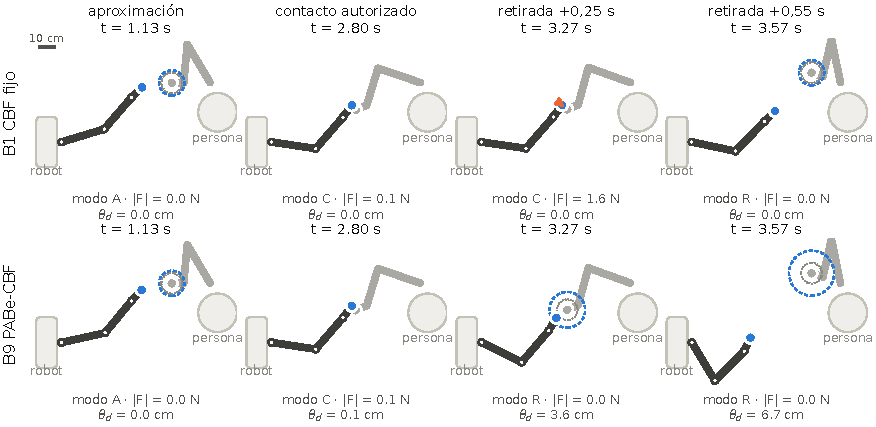
\includegraphics[width=\textwidth]{figures/fig_scene.pdf}
\caption{Episodio representativo de retirada durante el contacto (test, participante
4019, elegido automáticamente como el de mayor diferencia de fuerza pico B1$-$B9). Gris oscuro:
brazo del robot, con la palma en azul. Gris claro: brazo humano. Círculo discontinuo: margen
total $d^{\rm sep}+\epsilon_d+\theta_d$ fuera del contacto; punteado: $d^{\rm sep}$.
Flecha naranja: fuerza de interacción. B9 anticipa la retirada y libera antes. B1 sólo
libera por el tirón táctil explícito y es arrastrado (Fig.~\ref{fig:timeseries}d).}
\label{fig:scene}
\end{figure*}

\begin{figure*}[!t]
\centering
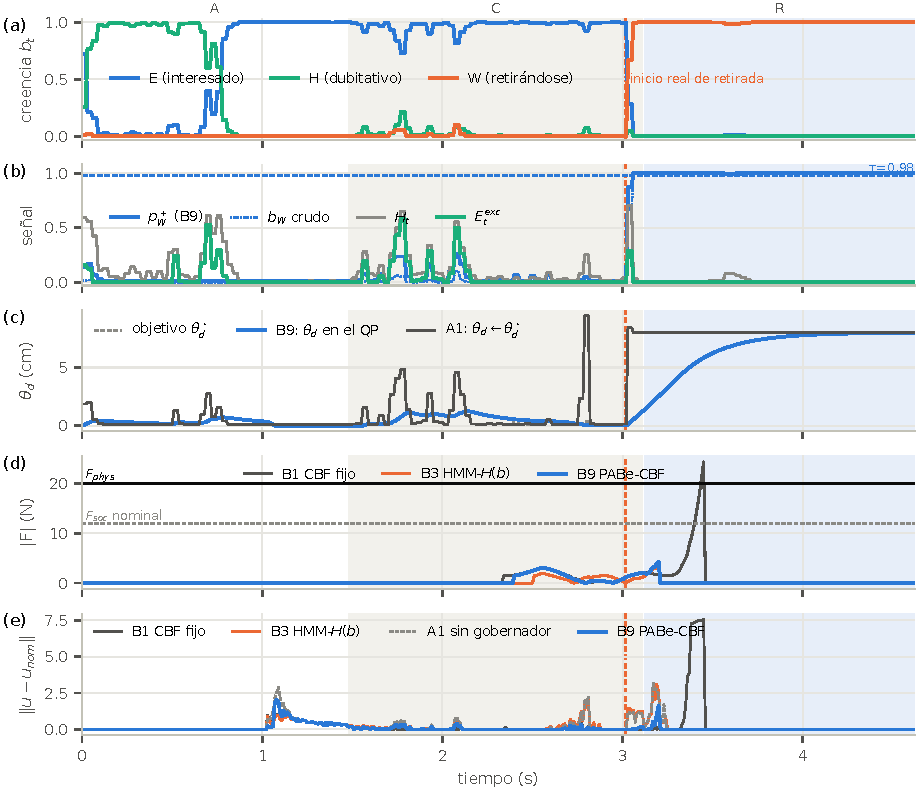
\includegraphics[width=\textwidth]{figures/fig_timeseries.pdf}
\caption{Señales internas en el episodio de la Fig.~\ref{fig:scene}. Sombreado: modo de
B9 (blanco: A; beige: C; azul: R). Línea naranja discontinua: inicio real de la retirada.
(a) Creencia del HMM. (b) $p_W^+$ frente a $b_W$, $H_t$ y $E^{\rm exc}_t$. Las
oscilaciones de entropía en la fase C no alcanzan el umbral de liberación.
(c) Margen $\theta_d$: el gobernador lo integra dentro del QP, mientras que en A1 salta
instantáneamente a $\theta_d^\star$. (d) Fuerza de interacción: B1 supera $F_{\rm phys}$.
(e) Corrección $\|u-u_{\rm nom}\|$: los saltos de $\theta$ en A1 y B3 producen
correcciones abruptas que B9 evita.}
\label{fig:timeseries}
\end{figure*}

\begin{table*}[!t]
\centering\footnotesize
\caption{Resultados en el test v2 (participantes no vistos). Porcentajes por episodio con IC 95\,\% de Clopper--Pearson. $F_{p95}$: percentil 95 de la fuerza pico por episodio. Sens.: retiradas detectadas por la regla semántica en $\le$1\,s. Infact.: episodios con $\ge$1 ciclo QP infactible.}
\label{tab:main}
\setlength{\tabcolsep}{3.2pt}
\resizebox{\linewidth}{!}{%
\begin{tabular}{lrrrrrrrrrr}
\toprule
Método & Viol. física \% & Cont. no aut. \% & $F_{p95}$ (N) & Lib. fallida \% & Sens. \% & Canc. falsa \% & Éxito \% & Infact. \% & Jerk p95 & $J_{int}$ \\
\midrule
B0 nominal & 54{,}8 \scriptsize[50{,}8, 58{,}9] & 47{,}3 & 15{,}4 & 10{,}9 \scriptsize[5{,}6, 18{,}7] & 0{,}0 & 10{,}3 \scriptsize[7{,}1, 14{,}3] & 89{,}7 & 0{,}0 & 176 & 0{,}000 \\
B1 CBF fijo & 4{,}3 \scriptsize[2{,}8, 6{,}3] & 0{,}0 & 19{,}7 & 15{,}7 \scriptsize[10{,}5, 22{,}1] & 0{,}0 & 8{,}7 \scriptsize[5{,}7, 12{,}4] & 91{,}3 & 22{,}3 & 326 & 0{,}294 \\
B2 HMM-MAP & 0{,}0 \scriptsize[0{,}0, 0{,}6] & 0{,}0 & 8{,}0 & 0{,}0 \scriptsize[0{,}0, 2{,}4] & 88{,}3 & 12{,}7 \scriptsize[9{,}1, 17{,}0] & 87{,}0 & 29{,}0 & 365 & 0{,}212 \\
B3 HMM-$H(b)$ ($\tau$=1{,}0) & 0{,}0 \scriptsize[0{,}0, 0{,}6] & 0{,}0 & 7{,}9 & 0{,}0 \scriptsize[0{,}0, 2{,}4] & 85{,}3 & 7{,}7 \scriptsize[4{,}9, 11{,}3] & 92{,}0 & 25{,}7 & 365 & 0{,}217 \\
B4 BCBF & 0{,}0 \scriptsize[0{,}0, 0{,}6] & 0{,}0 & 6{,}0 & 0{,}0 \scriptsize[0{,}0, 2{,}3] & 93{,}3 & 10{,}3 \scriptsize[7{,}1, 14{,}3] & 85{,}0 & 3{,}3 & 382 & 0{,}359 \\
B5 CRC-CBF ($\tau$=0{,}95) & 0{,}0 \scriptsize[0{,}0, 0{,}6] & 0{,}0 & 7{,}3 & 0{,}0 \scriptsize[0{,}0, 2{,}3] & 85{,}3 & 5{,}3 \scriptsize[3{,}1, 8{,}5] & 91{,}0 & 73{,}0 & 380 & 0{,}366 \\
B6 TV-CBF ($\tau$=0{,}98) & 0{,}0 \scriptsize[0{,}0, 0{,}6] & 0{,}0 & 8{,}1 & 0{,}0 \scriptsize[0{,}0, 2{,}3] & 82{,}3 & 6{,}3 \scriptsize[3{,}9, 9{,}7] & 93{,}7 & 6{,}7 & 349 & 0{,}204 \\
B7 SHIELD & 5{,}3 \scriptsize[3{,}7, 7{,}4] & 0{,}0 & 20{,}0 & 19{,}3 \scriptsize[13{,}6, 26{,}1] & 0{,}0 & 9{,}3 \scriptsize[6{,}3, 13{,}2] & 90{,}7 & 22{,}8 & 328 & 0{,}284 \\
B8 RCIP & 0{,}3 \scriptsize[0{,}0, 1{,}2] & 0{,}0 & 8{,}5 & 1{,}5 \scriptsize[0{,}2, 5{,}2] & 84{,}3 & 19{,}0 \scriptsize[14{,}7, 23{,}9] & 81{,}0 & 5{,}3 & 343 & 0{,}164 \\
B9 PABe-CBF ($\tau$=0{,}98) & 0{,}0 \scriptsize[0{,}0, 0{,}6] & 0{,}0 & 8{,}2 & 0{,}0 \scriptsize[0{,}0, 2{,}3] & 82{,}0 & 6{,}3 \scriptsize[3{,}9, 9{,}7] & 93{,}7 & 5{,}7 & 340 & 0{,}199 \\
\bottomrule
\end{tabular}}
\\[2pt]\parbox{\linewidth}{\scriptsize B0 sólo en simulación. B2, B4, B7 y B8 usan su regla nativa sin barrido de umbral; B3, B5 y B9 usan el umbral elegido en validación para igualar sensibilidad. Jerk en m/s$^3$; $J_{int}$ adimensional (normalizado por $u_{max}$).}
\end{table*}


\begin{figure*}[!t]
\centering
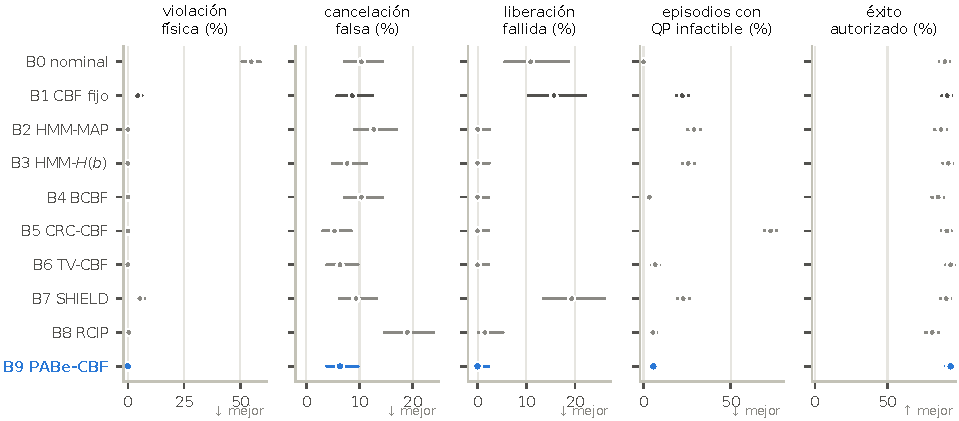
\includegraphics[width=\textwidth]{figures/fig_methods.pdf}
\caption{Resultados primarios por método en test (punto: tasa por episodio; barra:
IC~95\,\% Clopper--Pearson; $n=600$ episodios por método).}
\label{fig:methods}
\end{figure*}

\subsection{H1: gobernador de viabilidad}
\label{sec:sim:h1}
El contraste preregistrado para H1 enfrenta a B9 con B6, que usa las mismas señales y márgenes
variables, pero con una ley de evolución exógena. Frente a B6, B9 reduce los episodios con algún
ciclo QP infactible en 1{,}0~pp [$-$1{,}8, $-$0{,}3] ($p_{\rm Holm}=0{,}030$). También reduce el
jerk p95 de la palma en 8{,}9\,m/s$^3$ ($p_{\rm Holm}=0{,}002$) y la energía de intervención
($p_{\rm Holm}=0{,}002$), sin aumentar las violaciones físicas: ninguno de los dos registró violaciones (Tabla~\ref{tab:contrasts}).
La ablación A1, que asigna $\theta\leftarrow\theta^\star$ de forma instantánea, aísla el mismo mecanismo con
mayor contraste (Tabla~\ref{tab:ablation}, Fig.~\ref{fig:ablation}): eleva los episodios infactibles
en 19{,}3~pp y el jerk p95 en 33\,m/s$^3$. La Fig.~\ref{fig:timeseries}c,e muestra el
mecanismo: con margen instantáneo, cada pico de $\theta^\star$ se traduce en una
corrección abrupta, mientras que B9 desacelera el crecimiento de $\theta$. \textbf{H1 se apoya en
este banco de pruebas}, aunque frente a B6 el efecto es pequeño en magnitud.

\begin{table*}[!t]
\centering\footnotesize
\caption{Contrastes pre-registrados (diferencia B9 $-$ X). IC 95\,\% y $p$ bilateral por bootstrap pareado remuestreando participantes (4000 réplicas); $p_{Holm}$ corrige por multiplicidad sobre la familia completa.}
\label{tab:contrasts}
\setlength{\tabcolsep}{3.2pt}
\resizebox{\linewidth}{!}{%
\begin{tabular}{lllrrrrr}
\toprule
Hip. & Contraste & Métrica & Diferencia & IC 95\,\% & $p$ & $p_{Holm}$ & $n$ ep./part. \\
\midrule
H1 & B9 vs B6 & episodios con QP infactible & $-$1{,}00 pp & [$-$1{,}83, $-$0{,}33] & 0{,}006 & 0{,}030 & 600/20 \\
H1 & B9 vs B6 & jerk p95 (m/s$^3$) & $-$8{,}90 & [$-$11{,}11, $-$6{,}81] & $<$0{,}001 & 0{,}002 & 600/20 \\
H1 & B9 vs B6 & $J_{int}$ & $-$0{,}005 & [$-$0{,}008, $-$0{,}004] & $<$0{,}001 & 0{,}002 & 600/20 \\
H2 & B9 vs B3 & cancelación falsa & $-$1{,}33 pp & [$-$2{,}66, $-$0{,}33] & 0{,}025 & 0{,}100 & 300/20 \\
H2 & B9 vs B5 & cancelación falsa & 1{,}00 pp & [$-$0{,}34, 2{,}37] & 0{,}252 & 0{,}754 & 300/20 \\
H2 & B9 vs B3 & sensibilidad & $-$3{,}33 pp & [$-$5{,}73, $-$1{,}33] & $<$0{,}001 & 0{,}002 & 300/20 \\
H3 & B9 vs B1 & violación de eslabón & 0{,}00 pp & [0{,}00, 0{,}00] & 1{,}000 & 1{,}000 & 600/20 \\
H3 & B9 vs B1 & contacto no autorizado & 0{,}00 pp & [0{,}00, 0{,}00] & 1{,}000 & 1{,}000 & 600/20 \\
H3 & B9 vs B1 & violación física (cualquiera) & $-$4{,}33 pp & [$-$6{,}00, $-$2{,}83] & $<$0{,}001 & 0{,}002 & 600/20 \\
\bottomrule
\end{tabular}}
\end{table*}


\subsection{H2: riesgo separado de la entropía}
\label{sec:sim:h2}
La Fig.~\ref{fig:frontier} muestra las fronteras riesgo--utilidad. En test, las curvas de B3,
B9 y A8 se superponen dentro de la incertidumbre. B5 alcanza mayor sensibilidad en la zona de baja cancelación,
pero a costa de un 73\,\% de episodios con QP infactible: su margen conforme contextual
salta al cambiar de modo. En los puntos elegidos en validación (Tabla~\ref{tab:h2}), B9 cancela
1{,}3~pp menos que B3, con IC [$-$2{,}7, $-$0{,}3], $p=0{,}025$ y $p_{\rm Holm}=0{,}10$. Ese punto, sin embargo, también
tiene 3{,}3~pp \emph{menos} sensibilidad ($p_{\rm Holm}=0{,}002$), por lo que la ventaja
desaparece al leerla sobre la frontera. Frente a B5 la diferencia no es significativa
(+1{,}0~pp; $p_{\rm Holm}=0{,}75$). La ablación A2, que sustituye $E^{\rm exc}$ por $H(b)$, tampoco
cambia las cancelaciones. \textbf{H2 no se apoya}. En este banco, una vez que la
creencia está bien especificada, ni la separación $p_W^+$/$E^{\rm exc}$ ni la entropía
excedente reducen las liberaciones falsas frente a una regla combinada $b_W+\lambda H$ con
umbral ajustado. Las versiones previas con un HMM mal especificado mostraron
diferencias mayores en ambos sentidos. Esto indica que la calidad del
modelo de creencia pesa más que la forma de la regla.

\begin{figure*}[!t]
\centering
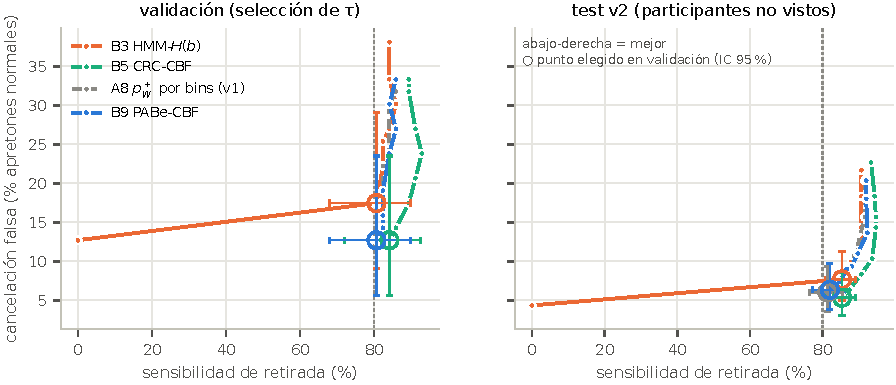
\includegraphics[width=\textwidth]{figures/fig_frontier.pdf}
\caption{Fronteras riesgo--utilidad al barrer el umbral de liberación $\tau$.
Sensibilidad: retiradas detectadas por la regla semántica en $\le1$\,s. Círculos:
puntos de operación elegidos en validación, con IC~95\,\%. Línea vertical: $s^\star=80$\,\%.}
\label{fig:frontier}
\end{figure*}

\begin{table}[!t]
\centering\footnotesize
\caption{Puntos de operación elegidos en validación para sensibilidad $\ge$ 80{,}0\,\% con mínima cancelación falsa, evaluados en test v2.}
\label{tab:h2}
\setlength{\tabcolsep}{3.2pt}
\resizebox{\linewidth}{!}{%
\begin{tabular}{lrrrrr}
\toprule
Método & $\tau$ & Sensibilidad \% & Cancelación falsa \% & Liberación fallida \% & Éxito \% \\
\midrule
B3 HMM-$H(b)$ & 1{,}0 & 85{,}3 \scriptsize[80{,}8, 89{,}1] & 7{,}7 \scriptsize[4{,}9, 11{,}3] & 0{,}0 \scriptsize[0{,}0, 2{,}4] & 92{,}0 \scriptsize[88{,}3, 94{,}8] \\
B5 CRC-CBF & 0{,}95 & 85{,}3 \scriptsize[80{,}8, 89{,}1] & 5{,}3 \scriptsize[3{,}1, 8{,}5] & 0{,}0 \scriptsize[0{,}0, 2{,}3] & 91{,}0 \scriptsize[87{,}2, 94{,}0] \\
A8 $p_W^+$ por bins & 0{,}98 & 81{,}3 \scriptsize[76{,}5, 85{,}6] & 6{,}0 \scriptsize[3{,}6, 9{,}3] & 0{,}0 \scriptsize[0{,}0, 2{,}3] & 94{,}0 \scriptsize[90{,}7, 96{,}4] \\
B9 PABe-CBF & 0{,}98 & 82{,}0 \scriptsize[77{,}2, 86{,}2] & 6{,}3 \scriptsize[3{,}9, 9{,}7] & 0{,}0 \scriptsize[0{,}0, 2{,}3] & 93{,}7 \scriptsize[90{,}3, 96{,}1] \\
\bottomrule
\end{tabular}}
\end{table}


\subsection{H3: barreras por eslabón y modo}
\label{sec:sim:h3}
Ningún método con barreras por eslabón (B1--B9) violó la separación de antebrazo,
muñeca o codo, ni produjo contacto no autorizado. Al sustituirlas por una única barrera
geométrica (A5), el 14{,}5\,\% de los episodios invade la separación de un eslabón no autorizado. A cambio,
el movimiento es más suave y hay menos infactibilidad, porque se imponen menos restricciones. Frente
a B1, B9 reduce las violaciones físicas totales en 4{,}3~pp ($p_{\rm Holm}=0{,}002$), gracias a
la liberación anticipada. \textbf{H3 se apoya}.

\begin{figure*}[!t]
\centering
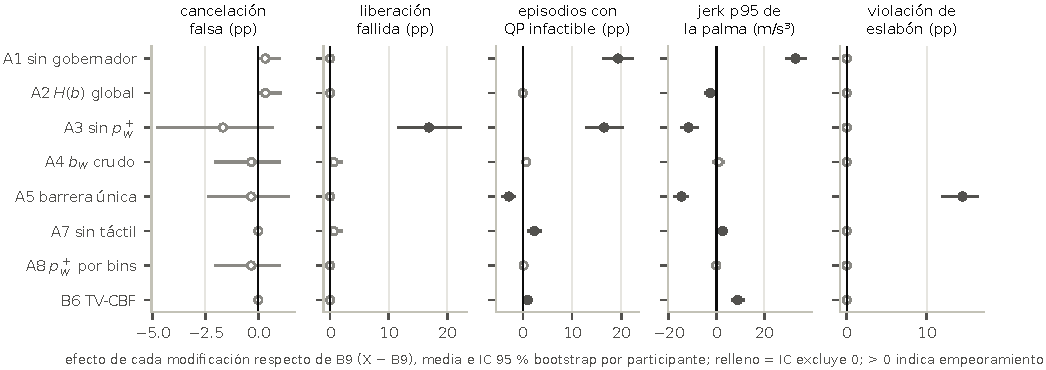
\includegraphics[width=\textwidth]{figures/fig_ablation.pdf}
\caption{Ablaciones: efecto de cada modificación respecto de B9 (X$-$B9) con IC~95\,\% por
bootstrap de participantes. Relleno: el IC excluye cero.}
\label{fig:ablation}
\end{figure*}

\begin{table*}[!t]
\centering\footnotesize
\caption{Ablaciones: efecto X $-$ B9 (pp o m/s$^3$) con IC 95\,\% bootstrap por participante; en negrita si el IC excluye 0. Valores positivos indican que eliminar el componente empeora la métrica.}
\label{tab:ablation}
\setlength{\tabcolsep}{3.2pt}
\resizebox{\linewidth}{!}{%
\begin{tabular}{lrrrrr}
\toprule
Variante & Canc. falsa & Lib. fallida & Ep. infactibles & Jerk p95 & Viol. eslabón \\
\midrule
A1 sin gobernador & 0{,}3 \scriptsize[0{,}0, 1{,}0] & 0{,}0 \scriptsize[0{,}0, 0{,}0] & \textbf{19{,}3 \scriptsize[16{,}3, 22{,}3]} & \textbf{33{,}0 \scriptsize[29{,}1, 37{,}0]} & 0{,}0 \scriptsize[0{,}0, 0{,}0] \\
A2 $H(b)$ global & 0{,}3 \scriptsize[0{,}0, 1{,}0] & 0{,}0 \scriptsize[0{,}0, 0{,}0] & 0{,}0 \scriptsize[0{,}0, 0{,}0] & \textbf{$-$2{,}6 \scriptsize[$-$4{,}4, $-$0{,}6]} & 0{,}0 \scriptsize[0{,}0, 0{,}0] \\
A3 sin $p_W^+$ & $-$1{,}7 \scriptsize[$-$4{,}7, 0{,}7] & \textbf{16{,}9 \scriptsize[11{,}7, 22{,}3]} & \textbf{16{,}5 \scriptsize[12{,}8, 20{,}2]} & \textbf{$-$11{,}6 \scriptsize[$-$14{,}6, $-$8{,}0]} & 0{,}0 \scriptsize[0{,}0, 0{,}0] \\
A4 $b_W$ crudo & $-$0{,}3 \scriptsize[$-$2{,}0, 1{,}0] & 0{,}6 \scriptsize[0{,}0, 2{,}0] & 0{,}7 \scriptsize[0{,}0, 1{,}3] & 1{,}0 \scriptsize[$-$1{,}0, 3{,}1] & 0{,}0 \scriptsize[0{,}0, 0{,}0] \\
A5 barrera única & $-$0{,}3 \scriptsize[$-$2{,}3, 1{,}4] & 0{,}0 \scriptsize[0{,}0, 0{,}0] & \textbf{$-$2{,}8 \scriptsize[$-$4{,}2, $-$1{,}7]} & \textbf{$-$14{,}6 \scriptsize[$-$17{,}5, $-$11{,}9]} & \textbf{14{,}5 \scriptsize[12{,}0, 16{,}3]} \\
A7 sin táctil & 0{,}0 \scriptsize[0{,}0, 0{,}0] & 0{,}6 \scriptsize[0{,}0, 1{,}9] & \textbf{2{,}3 \scriptsize[1{,}2, 3{,}7]} & \textbf{2{,}7 \scriptsize[1{,}4, 3{,}9]} & 0{,}0 \scriptsize[0{,}0, 0{,}0] \\
A8 $p_W^+$ por bins & $-$0{,}3 \scriptsize[$-$2{,}0, 1{,}0] & 0{,}0 \scriptsize[0{,}0, 0{,}0] & 0{,}2 \scriptsize[0{,}0, 0{,}5] & $-$0{,}1 \scriptsize[$-$1{,}1, 1{,}1] & 0{,}0 \scriptsize[0{,}0, 0{,}0] \\
B6 TV-CBF & 0{,}0 \scriptsize[0{,}0, 0{,}0] & 0{,}0 \scriptsize[0{,}0, 0{,}0] & \textbf{1{,}0 \scriptsize[0{,}3, 1{,}8]} & \textbf{8{,}9 \scriptsize[6{,}8, 11{,}1]} & 0{,}0 \scriptsize[0{,}0, 0{,}0] \\
\bottomrule
\end{tabular}}
\end{table*}


\subsection{Calibración de la señal de retirada}
\label{sec:sim:calib}
La cota isotónica v2 mejora la calidad probabilística frente a la versión por bins
(Tabla~\ref{tab:calibration}): ECE de 0{,}039 a 0{,}019, log-loss de 0{,}237 a 0{,}191 y AUROC de
0{,}874 a 0{,}956, es decir, recupera la capacidad de ordenamiento de $b_W$. Sin embargo, la
Fig.~\ref{fig:reliability} revela un resultado negativo importante. En test, con participantes nuevos y
un 25\,\% con cambio de dominio, $p_W^+$ \emph{no} es una cota superior uniforme. En los bins
0{,}1--0{,}4 la frecuencia observada de W supera la probabilidad predicha, aunque estos
bins reúnen sólo el 5\,\% de los ticks. La garantía marginal de calibración no se
transfiere bajo desplazamiento de dominio, como advertía la Sec.~3.2, y no debe
presentarse como cota condicional. En lazo cerrado, A8 y B9 no difieren en ninguna métrica
primaria al umbral elegido.

\begin{figure}[!t]
\centering
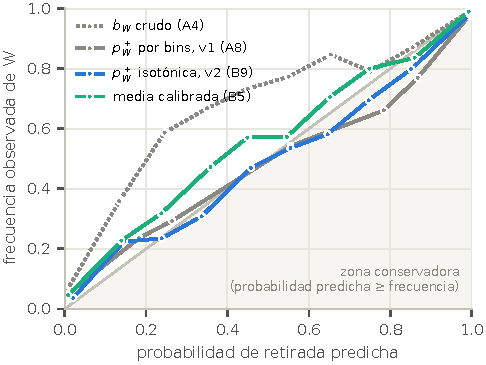
\includegraphics[width=\columnwidth]{figures/fig_reliability.pdf}
\caption{Diagrama de fiabilidad de la señal de retirada en test (10 bins, $\ge$20 ticks por bin).
Los puntos por encima de la diagonal indican subestimación del riesgo.}
\label{fig:reliability}
\end{figure}

\begin{table}[!t]
\centering\footnotesize
\caption{Calidad probabilística de la señal de retirada en test v2 (por tick; los ticks están autocorrelados, por lo que estas cifras son descriptivas). $p_W^+$ pretende ser una cota superior: un buen resultado es ECE bajo con sesgo conservador (ver Fig.~\ref{fig:reliability}).}
\label{tab:calibration}
\setlength{\tabcolsep}{3.2pt}
\resizebox{\linewidth}{!}{%
\begin{tabular}{lrrrrr}
\toprule
Señal & Brier & log-loss & ECE & AUROC & Recall@FPR5\% \\
\midrule
$b_W$ crudo (A4) & 0{,}060 & 0{,}297 & 0{,}055 & 0{,}959 & 0{,}821 \\
$p_W^+$ por bins, v1 (A8) & 0{,}055 & 0{,}237 & 0{,}039 & 0{,}874 & 0{,}825 \\
$p_W^+$ isotónica, v2 (B9) & 0{,}051 & 0{,}191 & 0{,}019 & 0{,}956 & 0{,}825 \\
media calibrada (B5) & 0{,}053 & 0{,}224 & 0{,}036 & 0{,}955 & 0{,}823 \\
\bottomrule
\end{tabular}}
\end{table}


\subsection{H4: coste computacional}
\label{sec:sim:h4}
La capa de seguridad completa de B9 (HMM, señales, autómata y QP conjunto) requiere
0{,}94/1{,}30/1{,}55\,ms en p50/p95/p99 por ciclo, con un máximo de 12{,}3\,ms. El QP conjunto
de 5 variables tarda 0{,}21\,ms en la mediana, frente a 0{,}17\,ms del QP de B1 con 3 variables
(Tabla~\ref{tab:latency}, Fig.~\ref{fig:latency}). Ningún ciclo de ningún método superó el
presupuesto de 150\,ms. Las cifras se midieron en Python con 14 procesos concurrentes y
\emph{no} incluyen adquisición, inferencia visual, transporte ni actuación, que en el sistema real
dominarán la latencia sensor$\to$actuador. \textbf{H4 se apoya sólo para el componente de
cómputo del filtro}.

\begin{figure}[!t]
\centering
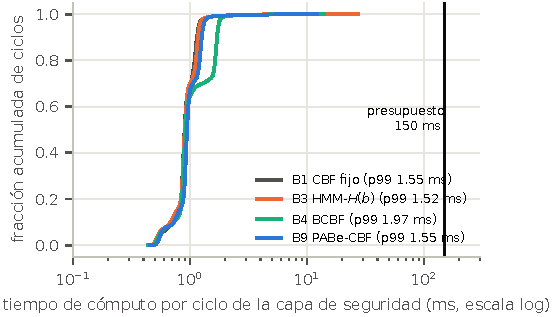
\includegraphics[width=\columnwidth]{figures/fig_latency.pdf}
\caption{Distribución acumulada del tiempo de cómputo por ciclo de la capa de seguridad.}
\label{fig:latency}
\end{figure}

\begin{table*}[!t]
\centering\footnotesize
\caption{Coste computacional por ciclo de la capa de seguridad (Python 3.12 + quadprog, un núcleo por proceso). No incluye adquisición, transporte ni actuación.}
\label{tab:latency}
\setlength{\tabcolsep}{3.2pt}
\resizebox{\linewidth}{!}{%
\begin{tabular}{lrrrrrrrr}
\toprule
Método & p50 & p95 & p99 & máx & QP p50 & QP p99 & HMM p50 & \% $>$150 ms \\
\midrule
B0 nominal & 0{,}256 & 0{,}526 & 0{,}657 & 35{,}99 & -- & -- & 0{,}233 & 0{,}00 \\
B1 CBF fijo & 0{,}900 & 1{,}190 & 1{,}549 & 12{,}09 & 0{,}170 & 0{,}278 & 0{,}230 & 0{,}00 \\
B2 HMM-MAP & 0{,}904 & 1{,}209 & 1{,}594 & 10{,}71 & 0{,}171 & 0{,}282 & 0{,}248 & 0{,}00 \\
B3 HMM-$H(b)$ & 0{,}903 & 1{,}210 & 1{,}516 & 27{,}11 & 0{,}171 & 0{,}256 & 0{,}254 & 0{,}00 \\
B4 BCBF & 0{,}913 & 1{,}748 & 1{,}970 & 13{,}88 & 0{,}171 & 0{,}250 & 0{,}764 & 0{,}00 \\
B5 CRC-CBF & 0{,}895 & 1{,}209 & 1{,}377 & 17{,}06 & 0{,}169 & 0{,}235 & 0{,}262 & 0{,}00 \\
B6 TV-CBF & 0{,}915 & 1{,}262 & 1{,}377 & 10{,}49 & 0{,}171 & 0{,}237 & 0{,}296 & 0{,}00 \\
B7 SHIELD & 1{,}058 & 1{,}347 & 1{,}492 & 15{,}87 & 0{,}172 & 0{,}246 & 0{,}228 & 0{,}00 \\
B8 RCIP & 0{,}896 & 1{,}186 & 1{,}309 & 11{,}20 & 0{,}170 & 0{,}237 & 0{,}242 & 0{,}00 \\
B9 PABe-CBF & 0{,}943 & 1{,}301 & 1{,}546 & 12{,}30 & 0{,}209 & 0{,}311 & 0{,}298 & 0{,}00 \\
\bottomrule
\end{tabular}}
\\[2pt]\parbox{\linewidth}{\scriptsize Tiempos en ms.}
\end{table*}

\begin{table*}[!t]
\centering\footnotesize
\caption{Desglose por familia de escenarios (test v2). Éxito: apretón completado si está autorizado y no hay retirada; ausencia de contacto si no está autorizado.}
\label{tab:families}
\setlength{\tabcolsep}{3.2pt}
\resizebox{\linewidth}{!}{%
\begin{tabular}{llrrrrr}
\toprule
Familia & Método & Viol. \% & $F$ pico medio (N) & Canc. falsa \% & Lib. fallida \% & Éxito \% \\
\midrule
(i) estable & B1 CBF fijo & 0{,}0 & 6{,}8 & 0{,}0 & -- & 100{,}0 \\
 & B3 HMM-$H(b)$ & 0{,}0 & 6{,}6 & 0{,}0 & -- & 100{,}0 \\
 & B5 CRC-CBF & 0{,}0 & 3{,}6 & 0{,}0 & -- & 99{,}0 \\
 & B9 PABe-CBF & 0{,}0 & 6{,}8 & 0{,}0 & -- & 100{,}0 \\
\midrule
(ii) retirada pre-contacto & B1 CBF fijo & 0{,}0 & 0{,}0 & -- & -- & 100{,}0 \\
 & B3 HMM-$H(b)$ & 0{,}0 & 0{,}0 & -- & -- & 100{,}0 \\
 & B5 CRC-CBF & 0{,}0 & 0{,}0 & -- & -- & 100{,}0 \\
 & B9 PABe-CBF & 0{,}0 & 0{,}0 & -- & -- & 100{,}0 \\
\midrule
(iii) retirada en contacto & B1 CBF fijo & 6{,}0 & 13{,}2 & -- & 6{,}0 & -- \\
 & B3 HMM-$H(b)$ & 0{,}0 & 3{,}6 & -- & 0{,}0 & -- \\
 & B5 CRC-CBF & 0{,}0 & 4{,}5 & -- & 0{,}0 & -- \\
 & B9 PABe-CBF & 0{,}0 & 5{,}5 & -- & 0{,}0 & -- \\
\midrule
(iv) duda inocua & B1 CBF fijo & 0{,}0 & 6{,}3 & 11{,}0 & -- & 89{,}0 \\
 & B3 HMM-$H(b)$ & 0{,}0 & 5{,}6 & 10{,}0 & -- & 90{,}0 \\
 & B5 CRC-CBF & 0{,}0 & 3{,}5 & 6{,}0 & -- & 85{,}0 \\
 & B9 PABe-CBF & 0{,}0 & 5{,}5 & 7{,}0 & -- & 93{,}0 \\
\midrule
(v) oclusión/táctil tardío & B1 CBF fijo & 2{,}0 & 6{,}3 & 26{,}8 & 20{,}0 & 73{,}2 \\
 & B3 HMM-$H(b)$ & 0{,}0 & 4{,}0 & 23{,}2 & -- & 76{,}8 \\
 & B5 CRC-CBF & 0{,}0 & 2{,}6 & 17{,}9 & 0{,}0 & 80{,}4 \\
 & B9 PABe-CBF & 0{,}0 & 4{,}4 & 21{,}4 & 0{,}0 & 78{,}6 \\
\midrule
(vi) perturbación & B1 CBF fijo & 18{,}0 & 12{,}5 & 0{,}0 & 32{,}1 & 100{,}0 \\
 & B3 HMM-$H(b)$ & 0{,}0 & 6{,}8 & 0{,}0 & 0{,}0 & 97{,}7 \\
 & B5 CRC-CBF & 0{,}0 & 6{,}6 & 0{,}0 & 0{,}0 & 100{,}0 \\
 & B9 PABe-CBF & 0{,}0 & 7{,}6 & 0{,}0 & 0{,}0 & 100{,}0 \\
\bottomrule
\end{tabular}}
\end{table*}


\subsection{Amenazas a la validez de la evaluación}
\label{sec:sim:threats}
\begin{enumerate}[label=(\roman*)]
\item La simulación es planar y cinemática, sin dinámica de cuerpo completo ni contacto
deformable. Los resultados no implican transferencia al G1.
\item El humano sigue un guion de lazo abierto y no reacciona al robot, salvo en el cierre.
\item El modelo de observación es sintético y lo diseñaron los mismos autores que el HMM, lo que
favorece a todos los métodos basados en creencia frente a B1 y B7.
\item B4, B5, B7 y B8 son adaptaciones mínimas de los trabajos citados y no
reproducciones. Además, B2, B4 y B8 no se barrieron en umbral.
\item El conjunto de validación se reutilizó entre la v1 y la v2, de modo que sólo la partición
de test es completamente nueva.
\item Las métricas de predicción se calculan por tick y están autocorrelacionadas.
\item La latencia medida excluye la percepción.
\end{enumerate}

\subsection{Síntesis}
\label{sec:sim:summary}
En este banco de pruebas, la contribución defendible de PABe-CBF es el
\emph{gobernador de viabilidad}: optimizar $\dot\theta$ conjuntamente con $u$ reduce la
infactibilidad y la brusquedad sin coste de seguridad y con un sobrecoste de cómputo de
$\approx$0{,}04\,ms por ciclo. También queda apoyada la \emph{separación por eslabón y modo} (H3), así como la utilidad de una
señal explícita de riesgo de retirada para evitar liberaciones fallidas (A3: +16{,}9~pp). No se
encontró evidencia de que separar $p_W^+$ de la entropía excedente reduzca las cancelaciones falsas frente a
una regla basada en entropía con umbral ajustado (H2). La cota calibrada $p_W^+$ tampoco se mantuvo como cota superior uniforme bajo
cambio de dominio. Estos dos puntos deben reformularse o someterse a nuevas pruebas antes de presentarse como
aportaciones.

\end{document}
